% !TeX program = pdflatex
\documentclass[aspectratio=169]{beamer}

\usepackage[utf8]{inputenc}
\usepackage[T1]{fontenc}
\usepackage[spanish]{babel}
\usepackage{graphicx}
\usepackage{xcolor}
\usepackage{tikz}
\usepackage{hyperref}
\hypersetup{colorlinks=true,linkcolor=black,urlcolor=blue}

% EPSC color palette (as in manuals)
\definecolor{epsc:oscuro}{HTML}{280091}
\definecolor{epsc:medio}{HTML}{4C5CC5}
\definecolor{epsc:claro}{HTML}{3FCFD5}
\definecolor{epsc:verde}{HTML}{00B299}

% Theme
\usetheme{metropolis}

% Mostrar índice al inicio de cada sección (excepto la primera),
% remarcando la sección actual
\AtBeginSection[]{
  \ifnum\value{section}>1
    \begin{frame}{Contenido}
      \tableofcontents[currentsection]
    \end{frame}
  \fi
}

% Title metadata
\title{SimAS 3.0 descendente predictivo}
\subtitle{Simulador de analizadores sintácticos descendentes predictivos}
\author{D. Antonio Llamas García}
\date{\today}

% Logos (optional): comment out if not available
% \titlegraphic{
\includegraphics[height=1.2cm]{../TFG_Antonio_Llamas_Garcia__SimAS_3_0____Manual_Tecnico/img/LogotipoEPSC.pdf}}

\begin{document}

% Transparencia de presentación (similar a portada de manuales)
% Transparencia de presentación (portada estilo Manual Técnico, adaptada a 16:9)
\begin{frame}[plain]
  % Fondos e insignias como en la portada del manual técnico
  % Rutas a PDFs existentes en los manuales
  \begin{tikzpicture}[remember picture, overlay]
    % Esquinas decorativas: arriba a la derecha y abajo a la izquierda
    \node [anchor=north east, inner sep=0pt] at (current page.north east)
      {
\includegraphics[width=0.22\paperwidth]{../TFG_Antonio_Llamas_Garcia__SimAS_3_0____Manual_Tecnico/img/topRightCorner.pdf}};
    \node [anchor=south west, inner sep=0pt] at (current page.south west)
      {
\includegraphics[width=0.22\paperwidth]{../TFG_Antonio_Llamas_Garcia__SimAS_3_0____Manual_Tecnico/img/bottomLeftCorner.pdf}};
    % UCO + emblema escuela, desplazados al borde inferior derecho
    \node (uco) [anchor=south east, inner sep=0pt, xshift=-8mm, yshift=2mm] at (current page.south east)
      {
\includegraphics[height=0.8cm]{../TFG_Antonio_Llamas_Garcia__SimAS_3_0____Manual_Tecnico/img/uco_debajo.pdf}};
    \node [anchor=south east, inner sep=0pt, xshift=-8mm] at (uco.south west)
      {
\includegraphics[height=0.8cm]{../TFG_Antonio_Llamas_Garcia__SimAS_3_0____Manual_Tecnico/img/emblema-ing-informatica.pdf}};
  \end{tikzpicture}

  % Bloque central con logotipo EPSC y títulos en paleta EPSC
  \vspace*{-8mm}
  \centering
  {
\includegraphics[width=0.36\linewidth]{../TFG_Antonio_Llamas_Garcia__SimAS_3_0____Manual_Tecnico/img/LogotipoEPSC.pdf}\\[4mm]}
  {\Large\bfseries\textcolor{epsc:medio}{TRABAJO FIN DE GRADO}\\[2mm]}
  {\large\bfseries\textcolor{epsc:verde}{Grado en Ingeniería Informática}\\[0.5mm]
   \large\bfseries\textcolor{epsc:verde}{Especialidad de Computación}\\[4mm]}
  {\LARGE\bfseries\textcolor{epsc:oscuro}{SimAS 3.0 descendente predictivo}\\[0.5mm]
   \normalsize\bfseries\textcolor{epsc:oscuro}{Simulador de analizadores sintácticos descendentes predictivos}\\[4mm]}
  {\normalsize\textbf{\color{epsc:verde}{\today}}}
\end{frame}

% Datos del proyecto (similar a ficha inicial de los manuales)
\begin{frame}{Datos del proyecto}
  \begin{itemize}
    \item Título: SimAS 3.0 descendente predictivo. Simulador de analizadores sintácticos descendentes predictivos.
    \item Autor: D. Antonio Llamas García
    \item Directores: Prof. Dr. Antonio Araúzo Azofra; Prof. Dra. María Luque Rodríguez
    \item Centro: Escuela Politécnica Superior de la Universidad de Córdoba
  \end{itemize}
\end{frame}



% Índice general (después de la segunda transparencia y los datos del proyecto)
\begin{frame}{Contenido}
  \tableofcontents
\end{frame}

% 1. Introducción
\section{Introducción}
% 1. Introducción
\begin{frame}{Introducción}
  \begin{itemize}
    \item SimAS 3.0 es un simulador educativo para comprender cómo funciona el análisis sintáctico descendente predictivo (LL(1)).
    \item Permite crear y editar gramáticas de contexto libre, construir la tabla predictiva y seguir, paso a paso, la derivación y el árbol sintáctico generado.
    \item La aplicación ha evolucionado desde SimAS 1.0 y 2.0, con una interfaz renovada, pestañas inteligentes, generación de informes y soporte multiidioma.
  \end{itemize}
\end{frame}

\begin{frame}{Motivación y alcance}
  \begin{itemize}
    \item Se partía de una versión previa con problemas de consistencia y portabilidad. Esta versión los corrige y unifica la experiencia para que no se pierda información al navegar ni al guardar.
    \item El trabajo se centra en el análisis descendente predictivo: eliminación de recursividad y factorización cuando procede, cálculo fiable de First/Follow y construcción de la tabla LL(1).
    \item Además, se incorporan funciones de recuperación de errores, informes completos y compatibilidad en Windows, macOS y Linux.
  \end{itemize}
\end{frame}

\begin{frame}{Qué aporta SimAS 3.0}
  \begin{itemize}
    \item Una forma visual y dinámica de aprender LL(1): la derivación y el árbol se construyen en tiempo real.
    \item Un asistente guiado que acompasa los pasos clave (transformaciones, conjuntos y tabla) con explicaciones y representación clara.
    \item Una base estable y coherente para la docencia: interfaz limpia, pestañas para trabajar con varias vistas y documentación exportable.
  \end{itemize}
\end{frame}




% 2. Objetivos
\section{Objetivos}
% 2. Objetivos
\begin{frame}{Objetivo general}
  \begin{itemize}
    \item Construir una herramienta pedagógica sólida para entender y practicar el análisis sintáctico descendente predictivo (LL(1)), uniendo teoría y visualización paso a paso.
  \end{itemize}
\end{frame}

\begin{frame}{Objetivos específicos}
  \begin{itemize}
    \item Robustecer el flujo completo: transformaciones de gramáticas cuando proceda, cálculo correcto de Primero/Siguiente y construcción de la tabla predictiva LL(1) sin ambigüedades.
    \item Mejorar la experiencia de aprendizaje con un asistente claro y con derivación/árbol en tiempo real.
    \item Facilitar la práctica: edición de gramáticas, funciones de recuperación de errores y generación de informes.
  \end{itemize}
\end{frame}

\begin{frame}{Calidad del software}
  El proyecto persigue una mejora tangible en la calidad del software:
  \begin{itemize}
    \item \textbf{Consistencia}: datos y estado coherentes al navegar y al guardar.
    \item \textbf{Eficiencia}: cálculos y renderizados ágiles en equipos estándar.
    \item \textbf{Fiabilidad}: resultados deterministas y manejo sólido de errores.
    \item \textbf{Usabilidad}: interfaz limpia, asistente por pasos y mensajes claros.
    \item \textbf{Compatibilidad}: correcto funcionamiento con recursos y formatos esperados.
    \item \textbf{Portabilidad}: funcionamiento equivalente en Windows, macOS y Linux.
    \item \textbf{Mantenibilidad}: código modular, patrones conocidos y documentación.
    \item \textbf{Extensibilidad}: base preparada para nuevas funciones y vistas.
  \end{itemize}
\end{frame}

\begin{frame}{Resultados esperados}
  \begin{itemize}
    \item Experiencias de simulación consistentes, sin pérdidas de datos al navegar entre vistas.
    \item Portabilidad real (Windows, macOS y Linux) y una interfaz limpia basada en pestañas.
    \item Un soporte didáctico reutilizable en clase y para el autoestudio (PDF/HTML).
  \end{itemize}
\end{frame}




% 3. Antecedentes
\section{Antecedentes}
% 3. Antecedentes
\begin{frame}{De dónde venimos}
  \begin{itemize}
    \item SimAS 1.0 sentó las bases: editor de gramáticas y simulación de analizadores descendentes y ascendentes.
    \item SimAS 2.0 amplió funciones: validación automática, más control sobre tablas y errores, e informes; pero aparecieron problemas de consistencia y portabilidad.
  \end{itemize}
\end{frame}

\begin{frame}{Lecciones aprendidas}
  \begin{itemize}
    \item La docencia necesita una herramienta estable: sin pérdidas de estado ni resultados inconsistentes entre pasos.
    \item La visualización es clave: derivación y árbol ayudan a fijar conceptos, pero deben generarse de forma fiable.
    \item La experiencia debe ser fluida: trabajar con varias vistas/pestañas y generar informes de forma sencilla.
  \end{itemize}
\end{frame}

\begin{frame}{Qué aporta SimAS 3.0 respecto a 2.0}
  \begin{itemize}
    \item Correcciones en transformaciones, conjuntos Primero/Siguiente y construcción de la tabla predictiva LL(1).
    \item Derivación y árbol en tiempo real, incluyendo nodos \(\epsilon\), y gestión clara de errores.
    \item Interfaz con pestañas inteligentes, i18n y ejecución consistente en Windows, macOS y Linux.
  \end{itemize}
\end{frame}




% 4. Requisitos
\section{Requisitos}
% 4. Requisitos
\begin{frame}{Visión general}
  \begin{itemize}
    \item El sistema se organiza en cuatro bloques: editor de gramáticas, simulador LL(1), tutorial y ayuda.
    \item La información fluye desde la edición hasta la simulación, manteniendo siempre la gramática y los artefactos generados.
  \end{itemize}
\end{frame}

\begin{frame}{Requisitos funcionales}
  \begin{itemize}
    \item \textbf{Editor}: crear/cargar/guardar gramáticas; validar símbolos, producciones y símbolo inicial; consultar y generar informe de gramática.
    \item \textbf{Simulador}: Primero/Siguiente, tabla predictiva LL(1), funciones de recuperación de errores, simulación continua y paso a paso, derivación y árbol.
    \item \textbf{Documentación}: informes (PDF) y recursos de ayuda; tutorial accesible desde cualquier vista.
  \end{itemize}
\end{frame}

\begin{frame}{Requisitos no funcionales}
  \begin{itemize}
    \item \textbf{Usabilidad}: interfaz clara, asistente por pasos y mensajes comprensibles.
    \item \textbf{Fiabilidad}: resultados deterministas y control de errores en todas las operaciones.
    \item \textbf{Compatibilidad/Portabilidad}: funcionamiento equivalente en Windows, macOS y Linux.
    \item \textbf{Rendimiento}: respuesta fluida en cálculos y renderizado del árbol/derivación.
    \item \textbf{Mantenibilidad/Extensibilidad}: diseño modular con patrones (MVC, Strategy, Observer) y recursos i18n.
  \end{itemize}
\end{frame}

\begin{frame}{Requisitos de interfaz e información}
  \begin{itemize}
    \item Interfaz basada en pestañas con navegación padre–hijo y estados consistentes.
    \item Gramática estructurada (símbolos, producciones, símbolo inicial) y artefactos derivados (Primero/Siguiente, tabla, informe, derivación y árbol).
  \end{itemize}
\end{frame}




% 5. Diseño
\section{Diseño}
% 5. Diseño
\begin{frame}{Arquitectura general}
  \begin{itemize}
    \item Arquitectura modular con separación clara entre \emph{modelo}, \emph{lógica de análisis} y \emph{presentación}.
    \item Persistencia de artefactos de gramática para mantener consistencia: gramática, Primero/Siguiente, tabla predictiva LL(1), derivación y árbol.
    \item Interfaz basada en pestañas inteligentes (padre–hijo) para trabajar en paralelo sin perder el contexto.
  \end{itemize}
\end{frame}

\begin{frame}{Grupos de gramáticas y dependencias}
  \begin{itemize}
    \item Cada \textbf{editor} abre una gramática y forma un \emph{grupo lógico} con los \textbf{simuladores} lanzados desde él: comparten gramática y artefactos (Primero/Siguiente, tabla LL(1), derivación y árbol).
    \item Las dependencias se mantienen dentro del grupo: cambios en el editor se reflejan en los simuladores del mismo grupo de forma coherente.
    \item También es posible abrir \textbf{simuladores independientes} (sin editor activo). En ese caso, el simulador trabaja con una gramática seleccionada/importada sin crear dependencia con ningún editor.
  \end{itemize}
\end{frame}

\begin{frame}{Diseño de paquetes}
  \begin{itemize}
    \item \textbf{bienvenida}: pantalla inicial y acceso rápido a tareas frecuentes.
    \item \textbf{gramatica}: modelo de gramática y artefactos derivados (Primero/Siguiente, tabla LL(1), árbol, derivación).
    \item \textbf{editor}: edición/validación de gramáticas e informes.
    \item \textbf{simulador}: ejecución paso a paso/continua y visualización.
    \item \textbf{utils}: utilidades comunes y servicios de apoyo.
    \item \textbf{resources}: internacionalización (i18n), textos y recursos gráficos.
  \end{itemize}
\end{frame}

\begin{frame}{Patrones y principios}
  \begin{itemize}
    \item MVC para desacoplar modelo, lógica y vistas.
    \item Strategy para algoritmos de análisis y recuperación de errores.
    \item Observer para sincronizar vistas con cambios en el modelo.
    \item Principios SOLID para facilitar mantenibilidad y extensibilidad.
  \end{itemize}
\end{frame}

\begin{frame}{Interfaz y experiencia de uso}
  \begin{itemize}
    \item Flujo guiado: edición \(\rightarrow\) análisis \(\rightarrow\) simulación \(\rightarrow\) informe.
    \item \textbf{Grupos de gramáticas}: pestañas padre-hijo con gramática compartida, manteniendo sincronía de datos.
    \item \textbf{Simuladores independientes}: pueden abrirse sin editor; operan sobre una gramática elegida sin depender de una pestaña de edición.
    \item Vistas sincronizadas: cualquier cambio en la gramática del grupo actualiza artefactos y simulación.
    \item Internacionalización: recursos de texto separados y conmutables en tiempo de ejecución.
  \end{itemize}
\end{frame}




% 6. Pruebas
\section{Pruebas}
% 6. Pruebas
\begin{frame}{Pruebas: validación de gramática}
  Validación coherente de símbolos, producciones y símbolo inicial.
  \vspace{2mm}
  \begin{center}
    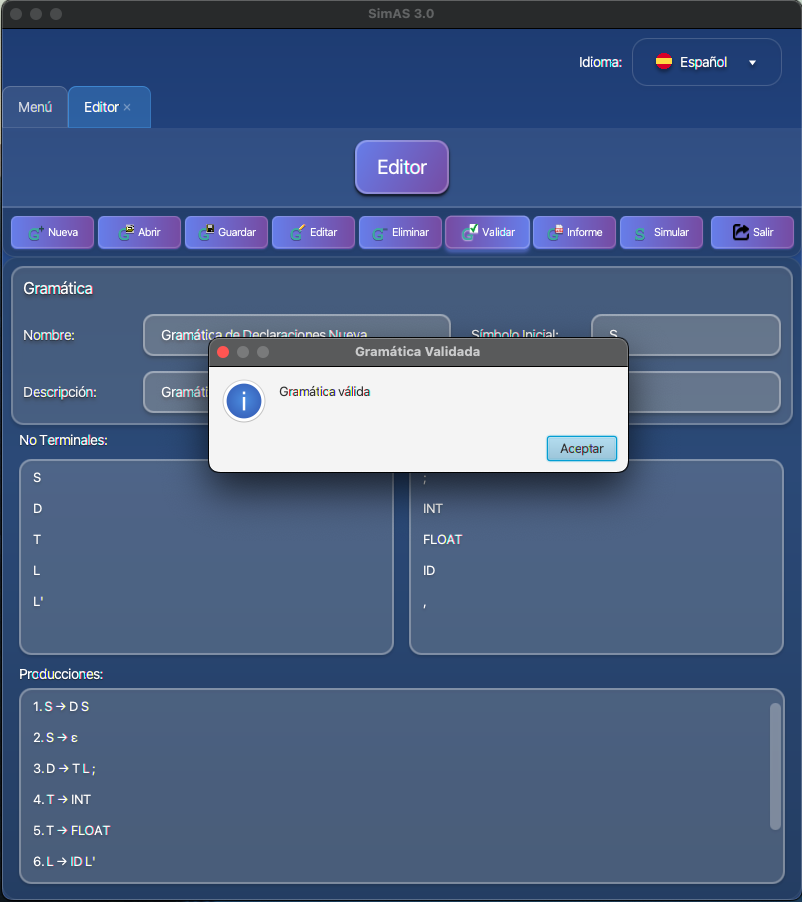
\includegraphics[width=0.98\linewidth,height=0.7\textheight,keepaspectratio]{../TFG_Antonio_Llamas_Garcia__SimAS_3_0____Manual_de_Usuario/figuras/editor/validar.png}
  \end{center}
\end{frame}

\begin{frame}{Pruebas: recursividad y factorización}
  Eliminación de recursividad izquierda y factorización correctas.
  \vspace{2mm}
  \begin{center}
    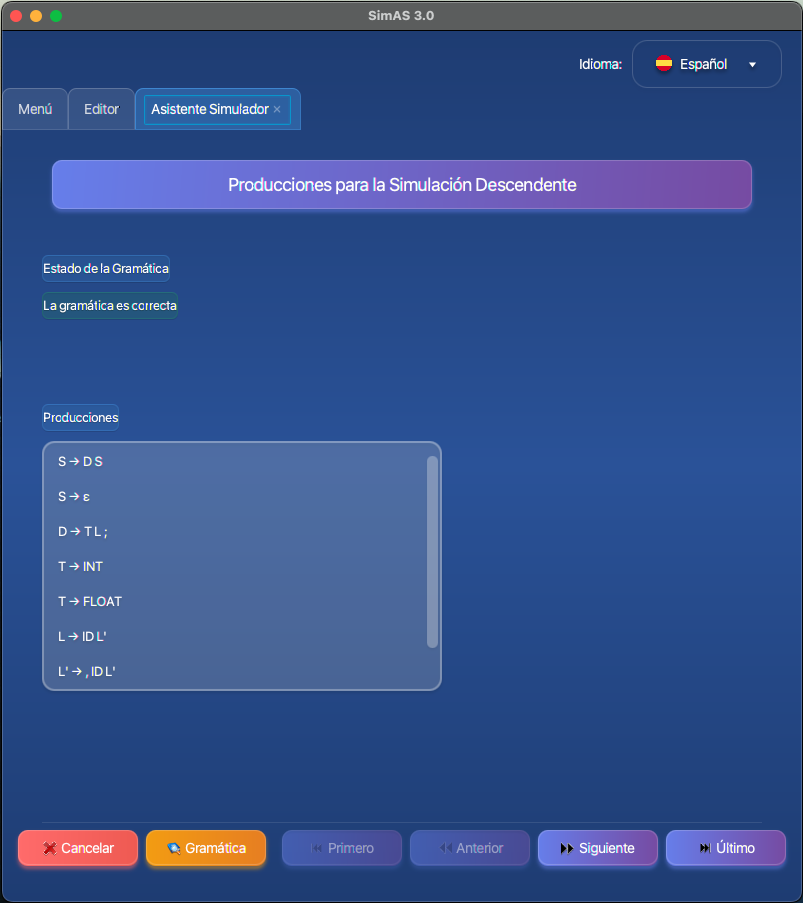
\includegraphics[width=0.98\linewidth,height=0.7\textheight,keepaspectratio]{../TFG_Antonio_Llamas_Garcia__SimAS_3_0____Manual_de_Usuario/figuras/simulador/paso1_recursividad_factorizacion.png}
  \end{center}
\end{frame}

\begin{frame}{Pruebas: conjuntos Primero/Siguiente}
  Cálculo estable y correcto de los conjuntos Primero/Siguiente.
  \vspace{2mm}
  \begin{center}
    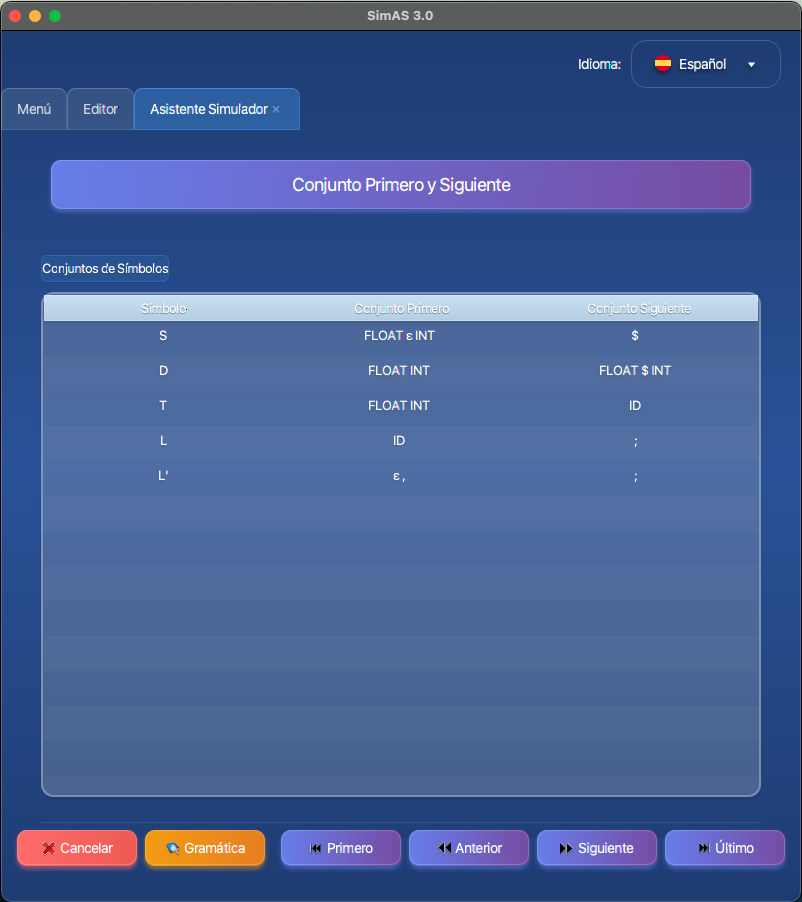
\includegraphics[width=0.98\linewidth,height=0.7\textheight,keepaspectratio]{../TFG_Antonio_Llamas_Garcia__SimAS_3_0____Manual_de_Usuario/figuras/simulador/paso2_conjuntos.png}
  \end{center}
\end{frame}

\begin{frame}{Pruebas: tabla predictiva LL(1)}
  Construcción de la tabla predictiva LL(1) sin ambigüedades.
  \vspace{2mm}
  \begin{center}
    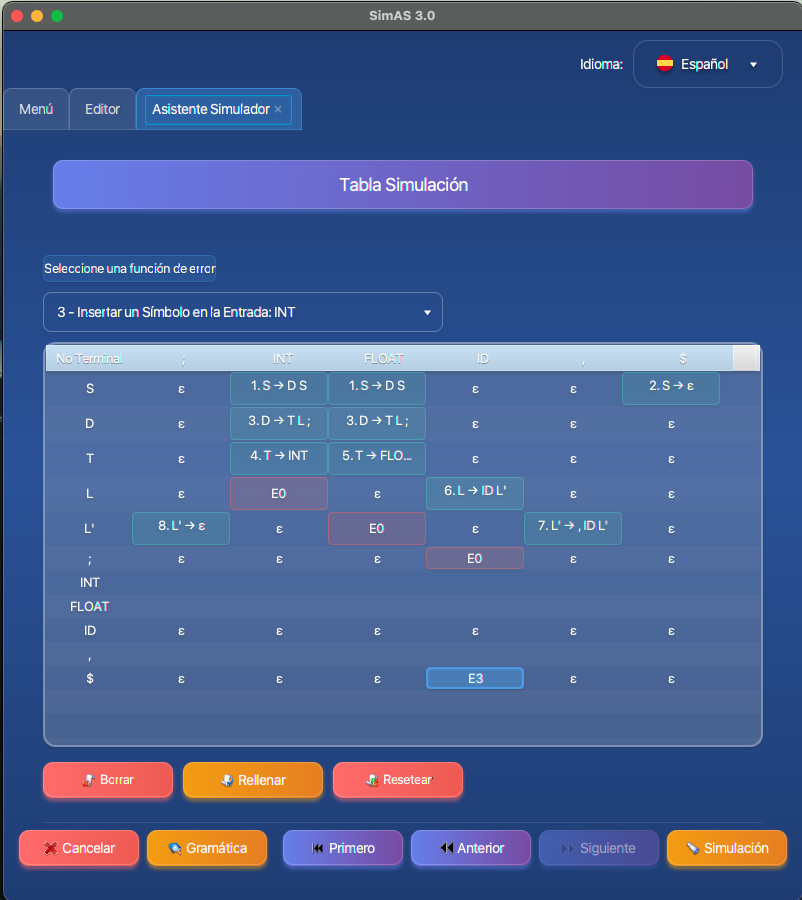
\includegraphics[width=0.98\linewidth,height=0.7\textheight,keepaspectratio]{../TFG_Antonio_Llamas_Garcia__SimAS_3_0____Manual_de_Usuario/figuras/simulador/paso5_tablaPredictivaCompleta.png}
  \end{center}
\end{frame}

\begin{frame}{Pruebas: funciones de recuperación de errores}
  Integración de funciones de error en la construcción y simulación.
  \vspace{2mm}
  \begin{center}
    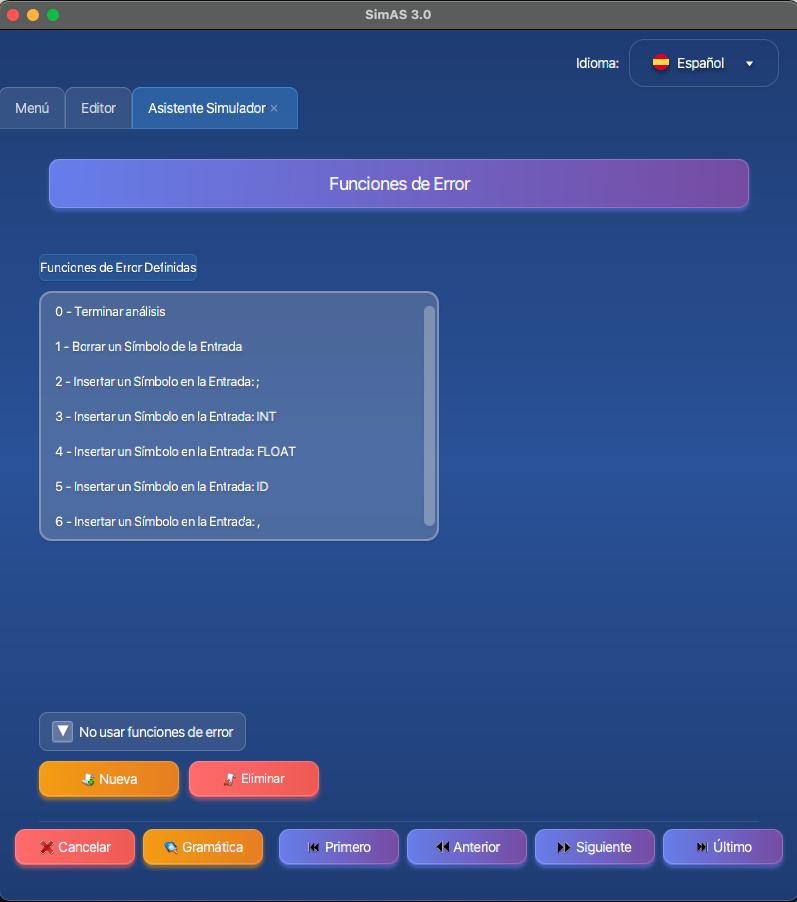
\includegraphics[width=0.98\linewidth,height=0.7\textheight,keepaspectratio]{../TFG_Antonio_Llamas_Garcia__SimAS_3_0____Manual_de_Usuario/figuras/simulador/paso4_funcionesError.png}
  \end{center}
\end{frame}

\begin{frame}{Pruebas: derivación paso a paso}
  Simulación determinista de la derivación de la cadena.
  \vspace{2mm}
  \begin{center}
    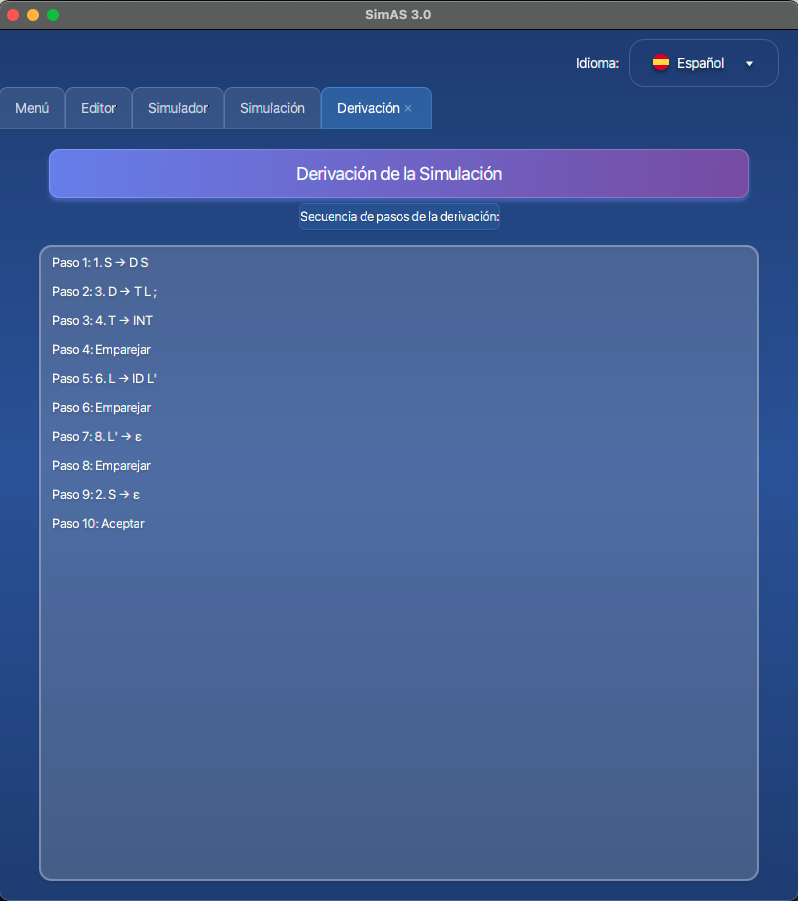
\includegraphics[width=0.98\linewidth,height=0.7\textheight,keepaspectratio]{../TFG_Antonio_Llamas_Garcia__SimAS_3_0____Manual_de_Usuario/figuras/simulador/simulacion_derivacion.png}
  \end{center}
\end{frame}

\begin{frame}{Pruebas: árbol sintáctico}
  Construcción del árbol sintáctico consistente con la derivación.
  \vspace{2mm}
  \begin{center}
    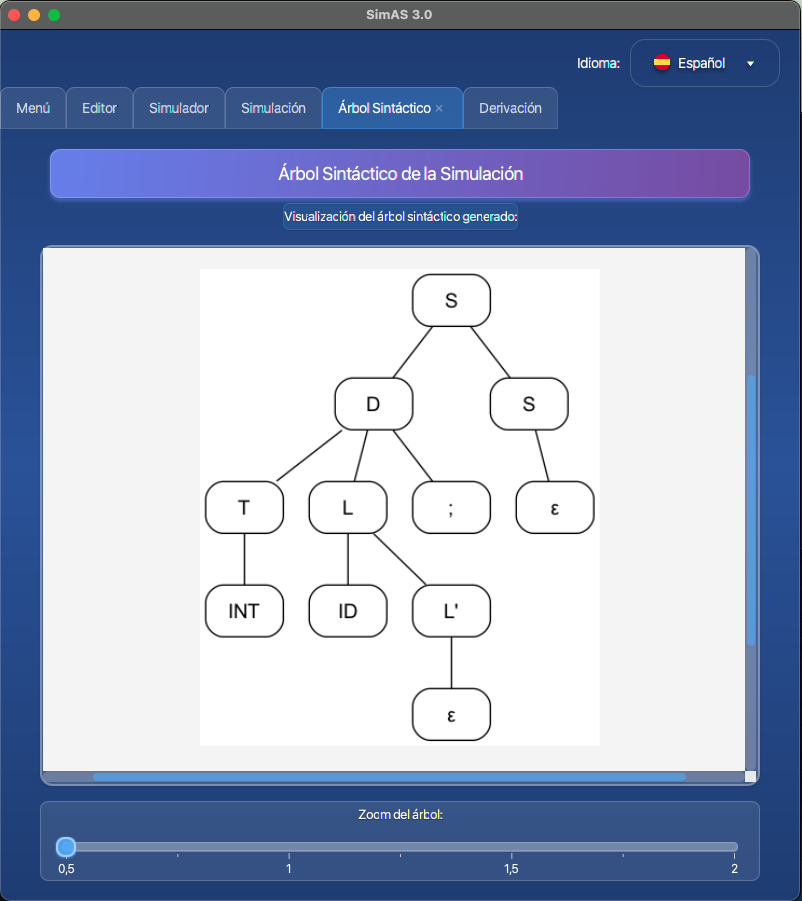
\includegraphics[width=0.98\linewidth,height=0.7\textheight,keepaspectratio]{../TFG_Antonio_Llamas_Garcia__SimAS_3_0____Manual_de_Usuario/figuras/simulador/simulacion_arbol.png}
  \end{center}
\end{frame}




% 7. Demostración del software
\section{Demostración del software}
% 7. Demostración del software
\begin{frame}[plain]
  \centering
  {\Huge \textbf{Demostración del software}}\\[6mm]
\end{frame}




% 8. Conclusiones
\section{Conclusiones}
% 8. Conclusiones
\begin{frame}{Conclusiones}
  \begin{itemize}
    \item SimAS 3.0 evoluciona la herramienta a un entorno pedagógico moderno centrado en análisis descendente predictivo.
    \item Se alcanza consistencia total: sin pérdidas de información entre módulos y resultados deterministas.
    \item Eficiencia y experiencia: menor consumo, respuesta ágil y navegación por pestañas más productiva.
  \end{itemize}
\end{frame}

\begin{frame}{Logros destacados}
  \begin{itemize}
    \item Correcciones clave: Primero/Siguiente y tabla predictiva LL(1) correctas; recursividad y factorización arregladas; informes fiables.
    \item Sisteme inteligente de navegación por pestañas que permite trabajar con varias gramáticas simultáneamente.
    \item Internacionalización dinámica y arquitectura modular (principios SOLID) para mantener y extender la aplicación.
  \end{itemize}
\end{frame}




% Fin (no incluir en índice)
% Fin
\begin{frame}[plain]
  \centering
  {\Huge \textbf{Fin}}\\[6mm]
  {\large Muchas gracias por la atención}
\end{frame}




\end{document}
